\documentclass[]{report}
\usepackage{fancyhdr}
\usepackage{longtable}
\usepackage{graphicx}
\usepackage{url}
\usepackage[semicolon]{natbib}
\usepackage{amsmath}
\usepackage{adjustbox}
\usepackage{babel,blindtext}
\usepackage{setspace}

\usepackage{tikz,pgfplots,pgf}
\usetikzlibrary{matrix,shapes,arrows,positioning}

\fancyhead{}
\fancyhead[LO, LE]{\rightmark}

\title{
	\begin{center}
	
\includegraphics[width=3cm]{assets/concordia-logo.png} \\
	\vspace{2mm}
	{Compatible-domain Transfer Learning for Breast cancer classification with limited Annotated Data} \\
	\vspace{5mm} %5mm vertical space
	\large {
		{Gina cody school of engineering and computer science}\\
		{Concordia University}\\
	}
    % change these details.
	\vspace{3mm} %3mm vertical space
	\textbf{ Masters in Applied Computer Science}\\
	{\large Module: Graduate Seminar Report}\\
	{\large Module Supervisor: Dr.Denis Pankratov}\\
	{\large Submission Date: 05/08/2022} \\
	\end{center}
}
\author{
	{\textbf{Speaker: Mohammad Amin Shamshiri}}\\
	{\large Report By:  Vinayak Sareen} \\
	{\large Student Id Number:  40186182} \\
}
\date{}
\pagestyle{fancy}
\begin{document}
\maketitle

\chapter*{Abstract}
this is the main abstract on what exactly i want to convey

\pagebreak
\section*{List of Abbreviation}
\begin{longtable}[c]{|c|c|c|}
    \hline
    1. & ANN & Artificial Neural Network \\
    \hline
    2. & CNN & Convolutional Neural Network \\
    \hline
    3. & GPU & Graphical Processing Unit \\
    \hline
    4. & WHO & World Health Organisation \\
    \hline
    5. & NHS & National Health Services in United Kingdom \\
    \hline
    6. & ConvNet & Convolutional Network \\ 
    \hline
    7. & ML & Machine Learning \\ 
    \hline
    8. & AI & Artificial Intelligence \\
    \hline
    9. & TL & Transfer Learning \\
    \hline
    10. & ROI & Region of interest \\
    \hline
\end{longtable}

% here we need to also have the list of symbols or the abbrevations. 
\tableofcontents
\onehalfspacing
\chapter{Introduction}
\section{Problem Statement}
The problem of breast cancer among women has been a major concern and leading cause of the mortality rate.
According to the WHO(World Health Organization) on the global scale around 502,000 cases of breast cancer among women are reported each year \citep*{jelen2008classification}. 
Furthermore, on the localized national scale, as per the anticipated reports from the Canadian cancer society, 28,600 women will be detected 
with malignant breast cancer, representing 25\% of the overall new cancer cases detected by the Canadian Cancer Society \citet{CanadianCancerSociety}.
\paragraph*{}
Moreover, according to the study conducted in the United Kingdom, the health care agency NHS had reported that 47\% trusts do not have the 
specialized nurses across the country. The lack of specialized medical staff members who can detect breast cancer at the early stage contributes to higher mortality rates \citep{tan2017breast}. 
The classical identification methods require the specialist to review the microscopic images of cytological images which is an inefficient manner even for the trained and qualified medical professionals with appropriate domain knowledge.
The problem can be solved using the automation with the CNN and implying the computer vision algorithms to provide the computer aided solution. Convolutional neural networks, 
which are specific kinds of artificial neural networks, extract data patterns 
from the images using the convolutional layers and further pass the extracted features to the fully connected 
layers of the network to learn the features \citep{wani2020basics}. However, such networks are highly reliant on the large volumes 
of the datasets with appropriate quality which is difficult to obtain in the real world systems. 


\pagebreak


% \section{Motivation/Application}
% this section contains the motivation to the topic BLAH BLAH BLAH
% \pagebreak

% \section{Objectives of Study}
% this section contains the problems associated to the topic BLAH BLAH BLAH
% \pagebreak

% \section{Assumptions and Limitations}
% this section contains the limitations associated with the project BLAH BLAH BLAH.
% \pagebreak

% \chapter{Background}
% \section{Traditional Breast Cancer Diagnosis Methods}
Trained pathologists diagnose breast cancer with specific facilities and equipment[ris wala]. The traditional clinical techniques used to classify breast cancer involve microarray, biopsy and cytology\citep{articlediagnosi}. 
The grading system proposed by the Dept of pathology across multiple universities based in India also suggests that a combination of clinical investigation, mammography and non-invasive methods can detect 99\% of cancers.
However, cytology is the specific diagnosis method that requires microscopic analysis of the specimens to differentiate between the malignant and benign tumours from the cytological images\citep{articlediagnosi}. 
The technique is used in binary cancer classification based on cytological images.

\section{Artificial Neural Networks}

\begin{center}
    \begin{figure}[htp]
        \centering
        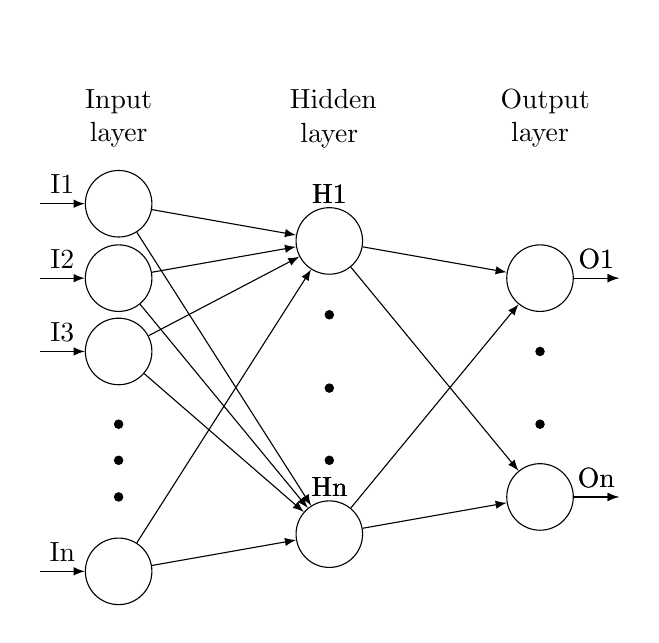
\begin{tikzpicture}[
        plain/.style={
          draw=none,
          fill=none,
          },
        dot/.style={draw,shape=circle,minimum size=3pt,inner sep=0,fill=black
          },
        net/.style={
          matrix of nodes,
          nodes={
            draw,
            circle,
            inner sep=8.5pt
            },
          nodes in empty cells,
          column sep=0.6cm,
          row sep=-11pt
          },
        >=latex
        ]
        \matrix[net] (mat)
        {
        |[plain]| \parbox{1cm}{\centering Input\\layer} 
                  & |[plain]| \parbox{1cm}{\centering Hidden\\layer} 
                               & |[plain]| \parbox{1cm}{\centering Output\\layer} \\
                  & |[plain]|                 \\
        |[plain]| &            & |[plain]|    \\
                  & |[plain]|  &              \\
        |[plain]| & |[dot]|                   \\
                  & |[plain]|  & |[dot]|      \\
        |[plain]| & |[dot]|    & |[plain]|    \\
        |[dot]|   & |[plain]|  & |[dot]|      \\
        |[dot]|   & |[dot]|    & |[plain]|    \\
        |[dot]|   & |[plain]|  &              \\
        |[plain]| &            & |[plain]|    \\
                  & |[plain]|                 \\
        };
        \foreach \ai/\mi in {2/I1,4/I2,6/I3,12/In}
          \draw[<-] (mat-\ai-1) -- node[above] {\mi} +(-1cm,0);
        \foreach \ai in {2,4,6,12}
        {\foreach \aii/\mii in {3/H1,11/Hn}
          \draw[->] (mat-\ai-1) -- (mat-\aii-2) node[yshift=0.6cm] {\mii};
        }
        \foreach \ai in {3,11}
        {  \draw[->] (mat-\ai-2) -- (mat-4-3);
          \draw[->] (mat-4-3) -- node[above] {O1} +(1cm,0);}
        \foreach \ai in {3,11}
        {  \draw[->] (mat-\ai-2) -- (mat-10-3);
          \draw[->] (mat-10-3) -- node[above] {On} +(1cm,0);}
        \end{tikzpicture}
        
        \caption{Multi Layered Neural Network diagram.}
        \caption{Drawing Credits: https://newbedev.com/drawing-neural-network-with-tikz}
        \label{fig_m_3}
        \end{figure}
\end{center}


There are various solutions for the classification problem some of them includes training the convolutional network, the section provides background on the artificial neural networks. The artificial neural networks also known as the ANN are 
biological inspired interconnected networks of neurons \citep{AGATONOVICKUSTRIN2000717}. 
The deep neural networks are based on the  perceptron based learning 
proposed by Frank Rosenblatt\citep{perceptron_learning}. The perceptron model had the limitation of only being applied to the linearly separable functions and therefore the deep neural networks were introduced\citep{perceptron_learning}
The neural networks are typically assigned with the weights at each layer, which are fine-tuned in the training phase of the model in order to minimize the cost function, which reflects the difference between 
the predicted classification value and actual value, the objective is to minimize the objective function also known as the cost function by updating the weights throughout the network\citep{perceptron_learning}
The typical neural network has various layers and each layer contains the set of neurons with the weights associated with the neurons from the various layers, the first layer of the network is known as the input layer, followed 
by various hidden layers and at last the output layer as shown in the fig[2.1] \citep{AGATONOVICKUSTRIN2000717}.

\subsection{Convolutional Neural Network }
\begin{center}
    \begin{figure}[!htp]
        \centering
        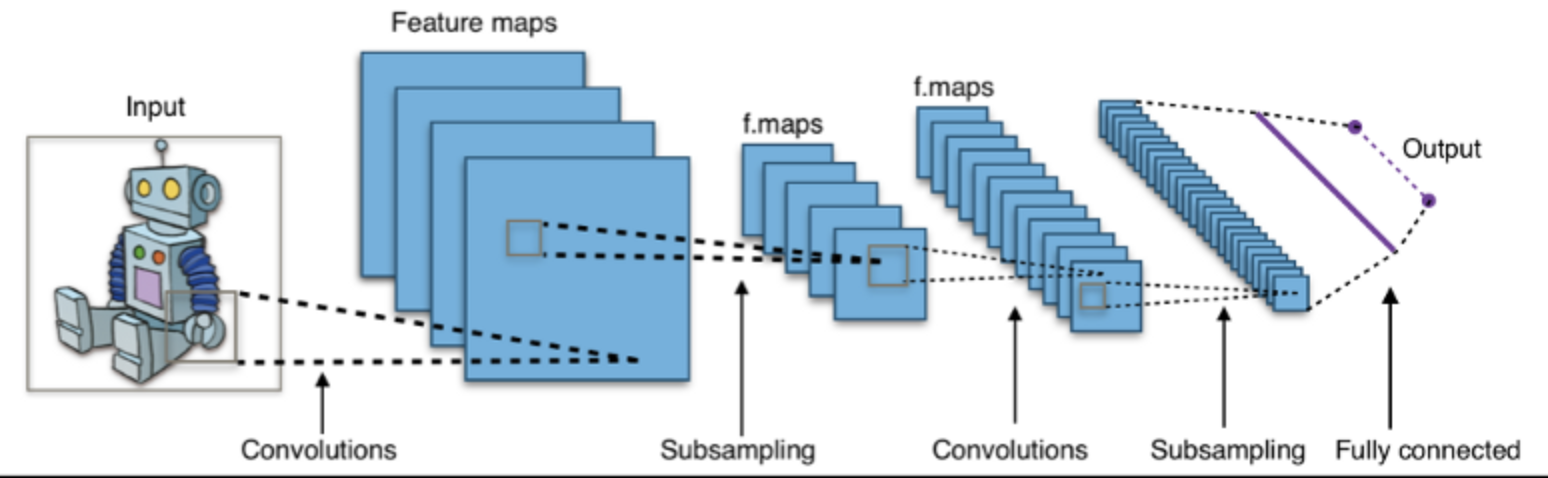
\includegraphics[keepaspectratio=true, scale=0.55]{assets/cnn-model_sample}
        \caption{Convolutional Neural Networks}
        \caption{Image Credits: $en.wikipedia.org/wiki/Convolutional_neural_network$}
        \label{fig:colorchannelseperation}
    \end{figure}
    
\end{center}

CNN are the special kinds of the neural networks which are generally used for the image recognition and image processing tasks[78]. The model intakes the image in the form of the pixels array with separate rgb channels and in order to extract the features from the images, the image kernels or convolutions are performed on the images to extract the feature maps[78]. Furthermore, the feature maps extracted from the convolutional layers are passed to the polling layer which downsamples the features resulting in the dimensionality reduction to the most prominent features in the images which are passed through the respective activation function chosen for the investigation. At the later layers, the feature maps are flattened and passed to the fully connected neural network explained in the previous[78]. 

\section{Transfer Learning}

\subsection{Why transfer learning is required}
The difficulty with training the ANN / CNN is that it is highly reliant on the huge dataset with high accuracy and precision for the training and validation phase,
which in real life scenario is difficult to obtain and cost ineffective solution. The convolutional neural networks also require hyper-parameter tuning.
in order to avoid the overfitting problem in the optimisation step of network training which is a time consuming process\citep{seldon}. 

\subsection{ How transfer-learning operates}

Transfer learning reuses experiential learning from pre-trained models which were trained to 
perform classification on similar dataset[99]. The pre-trained model's weights are used in the fine-tuning phase of the new model 
and therefore, it reduces the need for huge amounts of data to train the networks from scratch\citep{seldon}. 

\chapter{Technical contribution}
The suggested framework has a total of 8 phases in the classification pipeline which is mentioned in the image presented in table 1.0. The experiments were performed in three scenarios that included pre-training the transfer-learning models on the imageNet, hisbrek dataset and with the random weight initialization in order to evaluate the performance
of each of the models with both partial and complete fine-tuning applied to the target models.

\section{Image Segmention and Preprocessing}
The first phase, targets to obtain the segmented regions of interests from the target source image. 
In order to perform the image segmentation of the source images of 
histopathological images, the pre-processing procedure was performed which involves 
the following sub-procedures which includes color channel separation and 
image normalization and explained in the detailed manner.
\pagebreak
\subsection{Color Channel Seperation}
\begin{figure}[!htp]
    \centering
    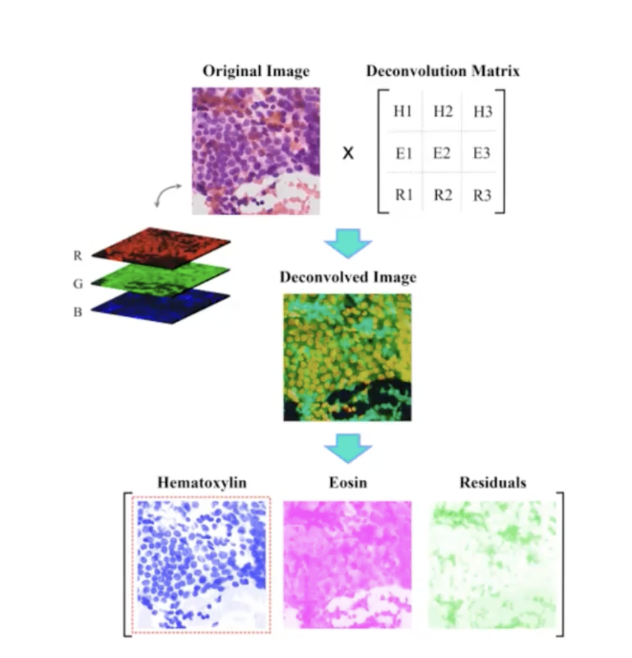
\includegraphics[scale=0.75]{assets/pre-processing.png}
    \caption{Image Credits: MSC Thesis Examination (Presentation) - Mohammad Amin Shamshiri}
\end{figure}
Color channel separation as shown in the figure[1.2] which aims at decomposing three color channels of the nucleus rather than the other components which are present within the image. In order to perform the color channel separation task, 
the deconvolutional matrix was applied to extract the feature maps of three distinct kinds that involve hematoxylin, Eosin and residuals. Upon investigation, the hematoxylin feature maps were most prominent and were used for the further normalization and segmentation. 


\subsection{Image normalization}
The normalization of the images are performed in order to ensure that the images are easier to process and each pixel in the image is normalized to range within 0 and 1 pixel values rather than 0 and 255, which is easier to train on the convolutional neural networks \citep{rashid_2019}.  

\subsection{Problems with using the UNET segmentation }
In the early phase of the experiments, the semantic segmentation was performed on the hematoxlyin images with an objective of grouping the each pixel in the images into the group of nuclei-interior, nuclei-edge or the background using the famous U-Net model, which requires the manual segmentation of the images and that is very time consuming process.
The subset of the original dataset was used to evaluate the performance of the segmented images upon splitting the dataset into the training and validation datasets respectively. 
However, the quantitative analysis of the U-Net segmentation was not possible and can only be evaluated on the visual basis. 
Therefore as for further investigation the intensity thresholding technique has been opted to deal with such problems and provide a reliable mechanism for image segmentation. 


\chapter{Conclusion}
\section{Conclusion}
Based on the experiments performed in the research, it is evident that transfer-learning using the domain compatible histopathological dataset provides high accuracy classification of the  cytological image sample. However, applying the partial fine-tuning to the context of the transfer learning is meaningful as compared to using the complete fine-tuning. The study also concludes that employing distinct CNN model architecture does not produce significant differences in the results except for the VGG-19 which performed worse than other models used in the context of transfer learning. The proposed framework yields 6-17\% improved accuracy when compared with the existing traditional machine learning solutions and  7\% compared to the solutions based on CNN methods.  Furthermore, the result of the study eliminates the needs for huge amounts of annotated data for the binary classification of the cytological images while providing the optimal results. The investigation has used a 17 times smaller dataset compared to the existing system while providing 3 per cent optimal results in terms of accuracy.

\section{Future Works}
In order to improve the existing framework, the speaker is looking forward to applying the multi-source domain adaptation techniques which will result in the minimizing the domain-shift between the source and target domain. Furthermore, the utilization of the light-weight network is also taken into consideration in order to  diminish the system’s dependence.  Atlast, the investigation will further be extended to be performed on the image-level scope instead of patch-level to evaluate the systems performance in classification of cancer malignancies in the patients. 


\bibliographystyle{IEEEtranN}
\bibliography{./references/references}
\pagebreak
\thispagestyle{plain}

\end{document}